\begin{frame}{Starting Simple: MLP Without Rules}
    \footnotesize
    \begin{columns}[T,onlytextwidth]
        \column{0.38\linewidth}
        \begin{itemize}
            \setlength\itemsep{0.35em}
            \item CasinoLimit~[1]: attack-related processes dataset, labeled
                  with \attack{} techniques.
            \item Convert each process into tokens.
            \item Predict the \attack{} technique from \textbf{local evidence only.}
        \end{itemize}

        \column{0.58\linewidth}
        \centering
        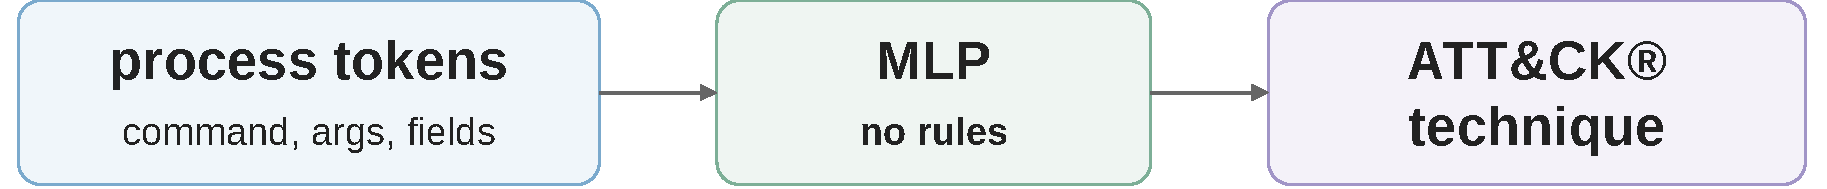
\includegraphics[width=\linewidth]{figures/diagrams/mlp_baseline.pdf}
    \end{columns}

    \vspace{-0.70em}
    \centering
    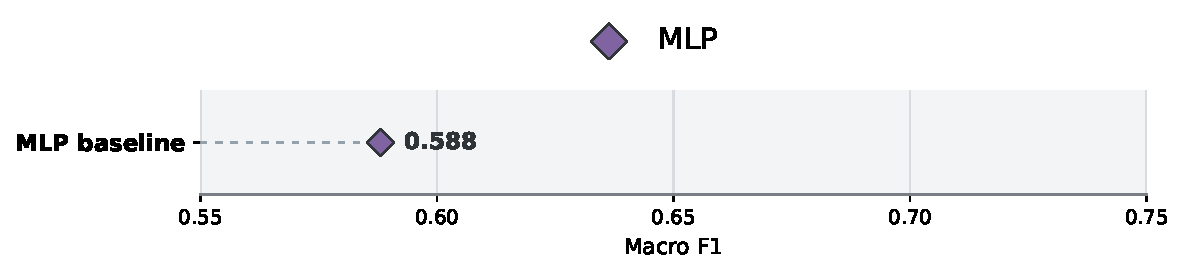
\includegraphics[width=0.80\linewidth]{figures/results/mlp_baseline_macro_f1.pdf}

    \vspace{-0.60em}
    {\tiny [1] S. Kilian et al., \emph{CasinoLimit: An Offensive Dataset Labeled with MITRE ATT\&CK Techniques}, RAID 2025.}
\end{frame}
